% Based off of the TEMPLATE for Usenix papers (https://www.usenix.org/sites/default/files/template.la_.txt)

\documentclass[letterpaper,twocolumn,10pt]{article}
\usepackage{usenix,epsfig,endnotes,hyperref,listings,textcomp}
\usepackage[T1]{fontenc}
\usepackage{algorithm}
%\usepackage{algorithmic}
\usepackage{algpseudocode}
\lstset{
	basicstyle=\footnotesize,
	breaklines=true,
	breakatwhitespace=true,
	escapechar=\%,
	numbers=left,
	tabsize=2,
	xleftmargin=2em
}

\begin{document}

%don't want date printed
\date{\today}

%make title bold and 14 pt font (Latex default is non-bold, 16 pt)
\title{\Large \bf Time Randomization to Thwart Concurrency Bug Exploitation}

%for single author (just remove % characters)
\author{
%{\rm Anonymized for Review}\\
%Do not distribute.
{\rm David M. Tagatac}\\
Columbia University
\and
{\rm Michalis Polychronakis}\\
Stony Brook University
%\and
%{\rm Tony Ling}\\
%Columbia University
\and
{\rm Salvatore J. Stolfo}\\
Columbia University
% copy the following lines to add more authors
% \and
% {\rm Name}\\
%Name Institution
} % end author

\maketitle
% Use the following at camera-ready time to suppress page numbers.
% Comment it out when you first submit the paper for review.
%\thispagestyle{empty}

\subsection*{Abstract}
Multithreaded programming is here to stay, and concurrency bugs are the focus of a growing number of attacks.
While most defensive efforts against such attacks seek to identify bugs during debugging, an alternative method seeks to make exploitation harder without the need to first identify the bugs - or even the fact that there are any.
Time randomization introduces more diversity among instances of the same software.
Because concurrency attacks inherently depend on the timing between and among threads, diversity in thread timing may decrease the chance that a successful attack on one system will succeed on another.

We study three implementations of time randomization, all using the injection of NOPs to alter program timing.  The results indicate that the overhead introduced by these implementations is impractically high.  However, the effectiveness of the method, especially when NOPs are injected before library function calls following synchronization points, indicates that more efficient time randomization is worth pursuing as a defense against concurrency attacks.

\section{Introduction}
With the pervasiveness of multicore architectures, multithreading is an important - and often necessary - tool when programming for performance.
However, programming with multiple threads is generally more difficult than programming for serial execution.
Each thread has the potential to contain any bug of a serial program, and on top of that, the uncertain interleaving of concurrent threads has the potential for concurrency bugs (e.g. data races).

Partial taxonomies of concurrency bugs have been constructed \cite{Farchi2003, Lu2008}, and it has been demonstrated that attacks on buggy multithreaded programs are a real concern \cite{Yang2012}.
Much of the effort in combating this threat has gone into tools and systems which detect data races in order to aid debugging \cite{Savage1997, Flanagan2004, Laadan2011, Pratikakis2011, Kasikci2013}.
An alternative approach is to guide multithreaded programs into memoized synchronization schedules \cite{Cui2010}.
This approach does not dwell on race detection, but rather on removing the nondeterminism from the portions of multithreaded programs where races are most likely.
However, schedule memoization in its most automated form is still susceptible to attack whenever the attacker can trigger a different schedule by changing the input.

We address the threat of concurrency attacks from yet another angle: automated software diversity.
Software homogeneity is dangerous in that it provides economies of scale to attackers \cite{Geer2003b}.
The relatively high cost of constructing an exploit for one bug is ameliorated by the opportunity to reuse that same exploit on every identical instance of the software.
As a result, automated software diversity is an active area of research for software in general \cite{Larsen2014}.
Concurrency vulnerabilities subject a homogenous world of software to the same dangers for the same reasons.

Our contribution is the experimental analysis of three implementations of automated software diversity through instruction level randomization via NOP injection:
\begin{enumerate}
	\item Injection of random-length NOP loops before every library function call.
	\item Injection of random-length NOP loops before every library function call immediately preceding a synchronization mechanism.
	\item Injection of random-length NOP loops before every library function call immediately following a synchronization mechanism.
\end{enumerate}

We find all three implementations above to be effective in reducing exploit success rates on both real bugs and canonical examples, ranging from X to X.  However, the overhead is too high to recommend these implementations as practical solutions.  We propose future directions for achieving the benefits of this defense without overhead, or with more tolerable overhead.

\section{Time Randomization}
\subsection{Threat Model}
The type of attack that time randomization seeks to thwart has the following properties:
\begin{itemize}
	\item The attack targets a concurrency bug.
	\item The attacker can gain knowledge about the relative timing between two or more threads relavent to the bug.
	\item The attacker leverages this knowledge to craft the attack.
\end{itemize}
Note that there are many ways to gain knowledge about relative thread timing, including results from fuzzing experiments.
In the case that the fuzzing is done on a binary, it may not even be obvious how many threads are involved.
Nevertheless, positive fuzzing results can be considered knowledge about relative thread timing which can then be used to craft an attack.

As an example, consider the following scenario:
A remote attacker is communicating with some server software, and has somehow become aware of a concurrency bug in that software.
He has devised a way to exploit the bug, which includes a method for inducing a buggy thread interleaving.
For concreteness, let's assume that the bug is exposed when a save operation is attempted by one thread during the critical section of another save operation in another thread (e.g. after some checking has been done, but before the results have been used, sometimes referred to as a time of check to time of use attack).
If the server immediately spawns threads to execute save operations in response to client requests, the attacker's work consists of identifying the proper delay between two save threads such that the critical sections intersect.
The critical sections in this context are sometimes referred to as a vulnerability window \cite{Yang2012}.

If the server software is available to the attacker, he can simply study it on a similar system (which he controls) to determine the appropriate delay required to expose the bug.
Armed with this knowledge, he stands a good chance of exploiting the bug on the target system by sending requests with the same delay.
\subsection{Automated Diversity}
Time randomization aims to make this type of attack much harder.
By making the relative timing between threads less predictable, the cost of carrying out the attack above is dramatically increased.

\section{Experimental Design}
To test both the efficacy and the performance of time randomization as a mechanism to thwart concurrency bug exploitation, we applied time randomization to two canonical and two real concurrency bugs.
\subsection{Canonical Bug: Nonatomic Code Region Assumed to be Atomic}
\cite{Farchi2003} presented a partial concurrency bug taxonomy, and \cite{Lu2008} later showed that in a narrow study of real world concurrency bugs, the vast majority are one of two types:
\begin{enumerate}
	\item Atomicity Violation: The desired serializability among multiple memory accesses is violated.
	\item Order Violation: The desired order between two memory accesses is flipped.
\end{enumerate}
To test time randomization on the first type, a simple concurrency bug was constructed mimicking a "nonatomic operations assumed to be atomic" programmer error.
\subsection{Canonical Bug: Order Violation}
TODO
\subsection{Real Bug: Libsafe CVE-2005-1125}
Libsafe is a library which protects processes against the exploitation of buffer overflow vulnerabilities in process stacks, as well as format string vulnerabilities.  It does this by intercepting all calls to C standard library functions known to be vulnerable, and then running ``safe" versions of those functions which issue warnings about exploit attempts before exiting without allowing the exploits to succeed.

A static global variable `dying' is used in Libsafe to indicate when an unsafe action has already been detected, and Libsafe is issuing warnings and exiting.  In this case, Libsafe stops checking for new exploit attempts.  However, this variable is not protected by any synchronization mechanisms, so in the case of a multithreaded program, the following sequence of events is possible:
\begin{enumerate}
	\item Thread A attempts an exploit.
	\item The exploit is caught by Libsafe, the `dying' flag is set, and Libsafe begins the warning and exit procedure.
	\item Thread B is scheduled, and attempts another exploit before Libsafe has exited thread A.
	\item Because the `dying' flag is set, thread B's exploit is not caught by Libsafe, and it succeeds.
\end{enumerate}
The proof-of-concept exploit (Figure \ref{fig_poc}) often realizes the above sequence of events, effectively bypassing Libsafe.
\begin{figure}
\lstinputlisting{libsafe-PoC.c}
\caption{The proof of concept exploit for concurrency bug CVE-2005-1125 \cite{CVE2005-1125}.  Both functions \texttt{func1} and \texttt{func2} attempt to overflow buffers in their own stack frames.  Either function running alone would be caught by Libsafe at the illegal calls to \texttt{strcpy}, but when run in parallel, the concurrency bug may allow one call to \texttt{strcpy} to succeed.}
\label{fig_poc}
\end{figure}
Time randomization was applied to Libsafe by interposing external library calls \cite{Conrad2009} made by Libsafe each with random numbers of inline assembly NOP instructions.  This was accomplished by first specifying a max delay (per interposition).  Then, for each of the external library functions that Libsafe uses, a random integer between zero and the max delay was selected.  Finally, that number was used as the loop limit on a loop of assembly NOPs for that external library function.  The interpositions of the NOP loops were compiled into a dynamic library file, and that file was specified to be preloaded with the LD\_PRELOAD environment variable.
The average time to make a (legal) \texttt{strcpy} function call, and the proof of concept exploit success rate were measured for several randomizations for each max delay ranging from 0 up to 50,000.  The dynamic library file used contains 64 external library calls made by Libsafe when the \texttt{strcpy} function is called.
\subsection{Real Bug: Libvirt CVE-2014-1447}

\section{Results}



\begin{figure}
\centering
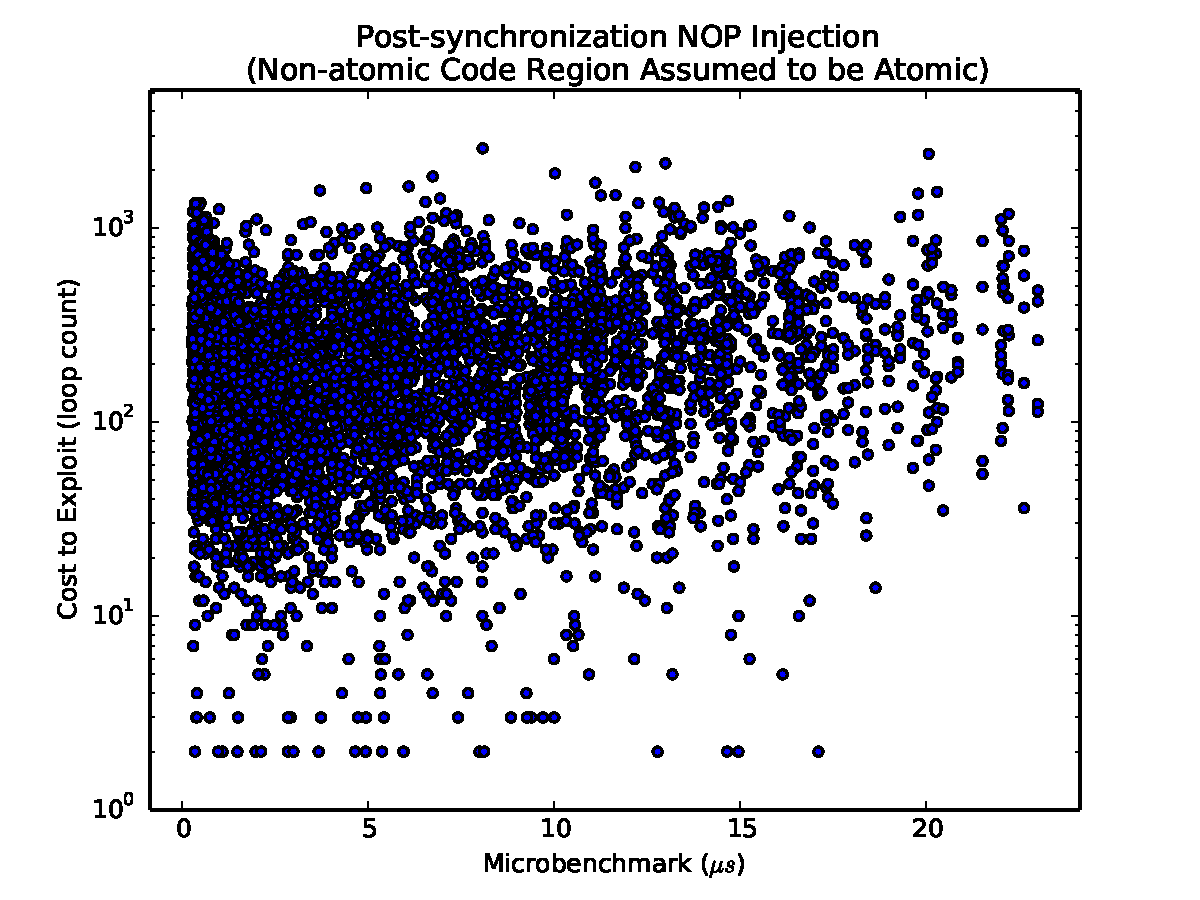
\includegraphics[width=\columnwidth]{figures/nonatomic-post}
\caption{Exploit cost (in number of exploit attempts) as a function of the microbenchmark after applying diversity implementation 3 to a canonical "nonatomic-region-assumed-to-be-atomic" concurrency bug.}
\label{fig_nonatomic-post}
\end{figure}

\begin{figure}
\centering
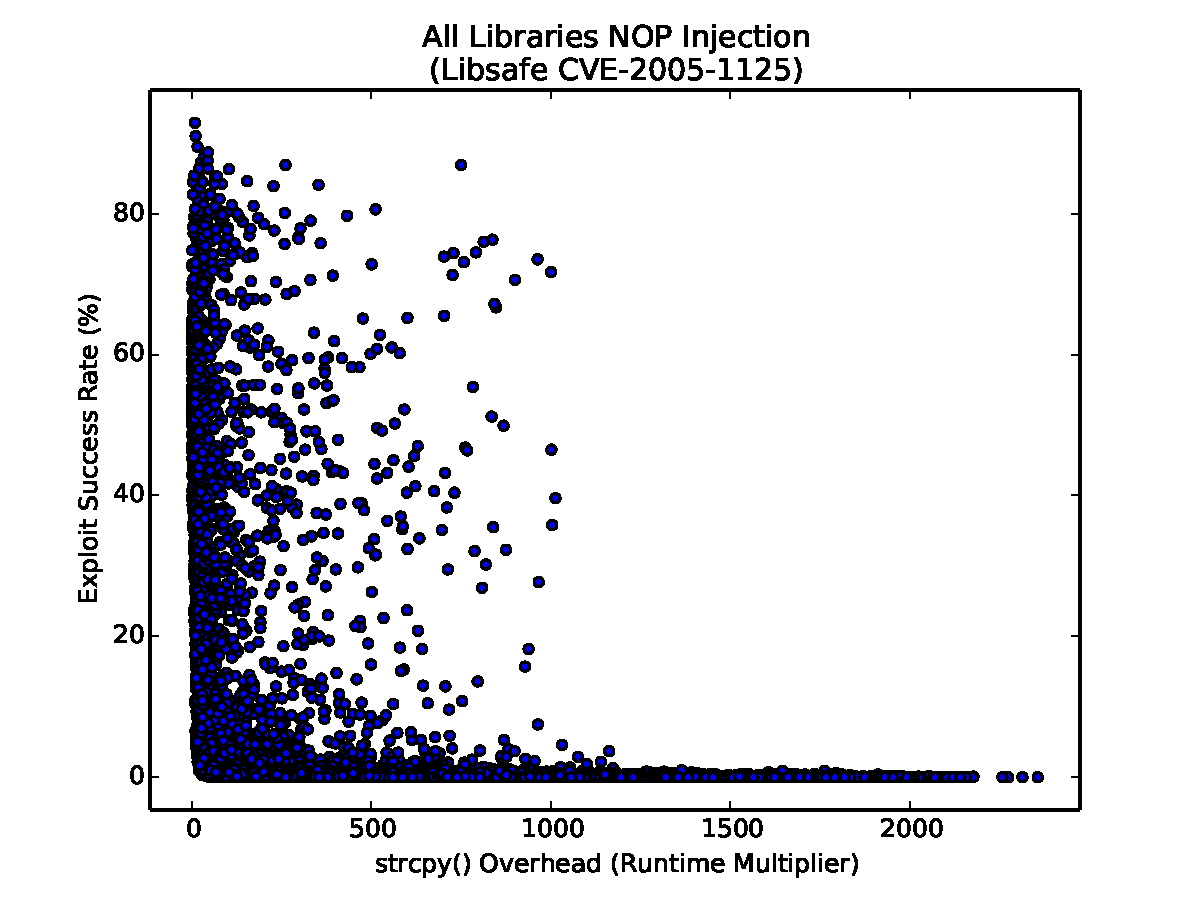
\includegraphics[width=\columnwidth]{figures/libsafe-all}
\caption{Exploit success rate as a function of the microbenchmark after applying diversity implementation 1 to Libsafe with concurrency bug CVE-2005-1125.}
\label{fig_libsafe-all}
\end{figure}

\begin{figure}
\centering
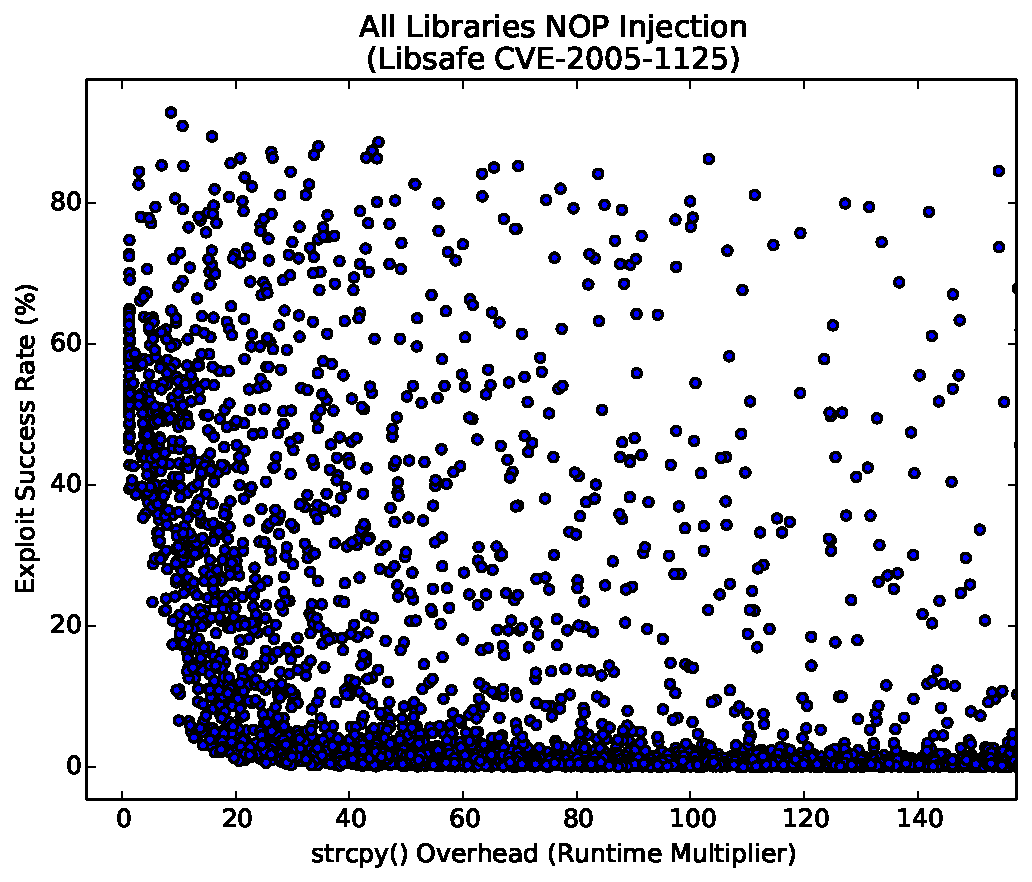
\includegraphics[width=\columnwidth]{figures/libsafe-all-zoom}
\caption{Exploit success rate as a function of the microbenchmark after applying diversity implementation 1 to Libsafe with concurrency bug CVE-2005-1125 (a zoom-in of Figure \ref{fig_libsafe-all}).}
\label{fig_libsafe-all-zoom}
\end{figure}

\begin{figure}
\centering
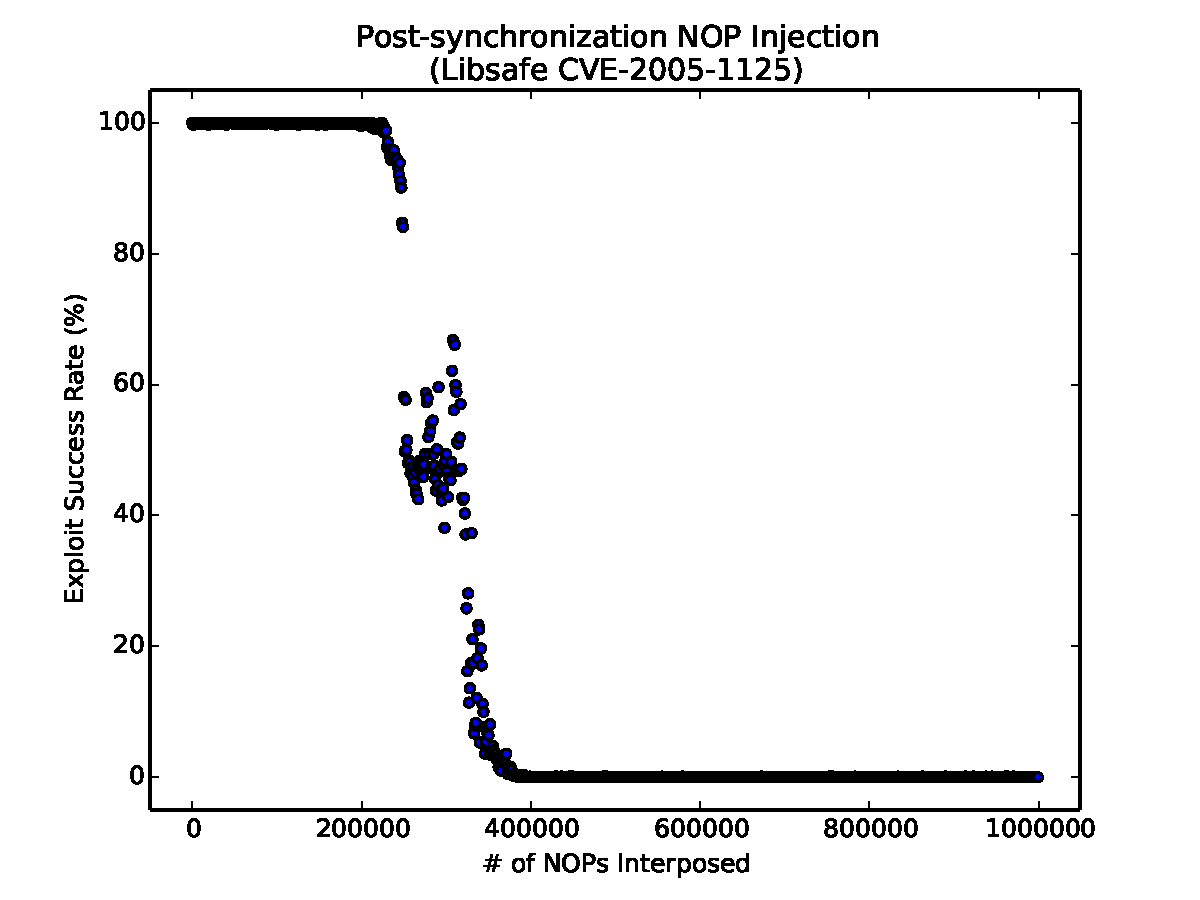
\includegraphics[width=\columnwidth]{figures/libsafe-post}
\caption{Exploit success rate as a function of the number of NOPs injected after applying diversity implementation 3 to Libsafe with concurrency bug CVE-2005-1125.}
\label{fig_libsafe-post}
\end{figure}

\begin{figure}
\centering
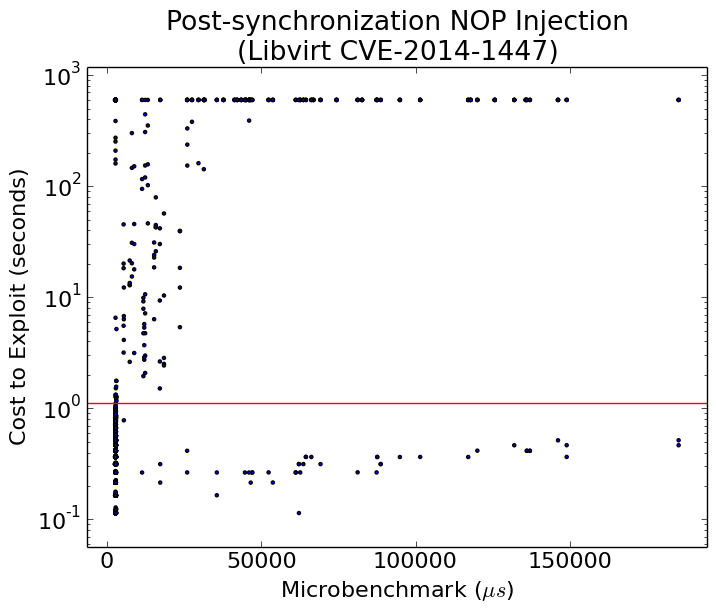
\includegraphics[width=\columnwidth]{figures/libvirt-post}
\caption{Exploit cost (in time) as a function of the microbenchmark after applying diversity implementation 3 to Libvirt with concurrency bug CVE-2014-1447.}
\label{fig_libvirt-post}
\end{figure}

\section{Future Directions}
TODO

\section{Related Work}
TODO

\section{Conclusion}
TODO

{\footnotesize \bibliographystyle{acm}
\bibliography{references}}

\end{document}


%%%%%%%%%%%%%%%%%%%%%%%%%%%%%%%%%%%%%%%%%%%%%%%%%%%%%%%%%%%%%%%%%%%%%%%%%%%%%%%%%%%%%%%%%%
%%%%%%%%%%%%%%%%%%%%%%%%%%%%%%%%%%%%%%%%%%%%%%%%%%%%%%%%%%%%%%%%%%%%%%%%%%%%%%%%%%%%%%%%%%
%\section{Introduction}
%Much like the way that address space layout randomization thwarts attacks that depend on absolute and/or relative code and data addresses in memory, we propose to thwart concurrency attacks that depend on specific thread timing by randomizing the delays between and among threads.  Like the memoization approach described above, we also focus on the synchronization schedule (the interleaving of the various threads in a multithreaded program).  However, instead of removing nondeterminism to increase reproducibility, we attempt to randomize the synchronization schedule to remove the possibility that the relative timing of two (or more) threads can be studied and used to craft an attack.  For this subset of concurrency attacks which depend on thread timing, we hypothesize that random injection of timing delays between concurrent threads will reduce the chance of any specific attack's success.  If such an attack can address different thread timing with correspondingly different input timing, at least randomization increases the cost to the attacker to determine the appropriate input timing; moreover, that knowledge is only useful for one system until the next randomization.
%
%\section{Time Randomization}
%Consider the following scenario: A remote attacker is communicating with some server software, and has somehow become aware of a concurrency bug in that software.  He has devised a way to exploit the bug, which includes a method for inducing a buggy thread interleaving.  For concreteness, let's assume that the bug is exposed when a save operation is attempted by one thread during the critical section of another save operation in another thread (e.g. after some checking has been done, but before the results have been used, sometimes referred to as a time of check to time of use attack).  If the server immediately spawns threads to execute save operations in response to client requests, the attacker's work consists of identifying the proper delay between two save threads such that the critical sections intersect.  The critical sections in this context are sometimes referred to as a vulnerability window \cite{Yang2012}.
%
%If the server software is available to the attacker, he can simply study it on a similar system (which he controls) to determine the appropriate delay required to expose the bug.  Armed with this knowledge, he stands a good chance of exploiting the bug on the target system by sending requests with the same delay.
%
%Time randomization aims to make this type of attack much harder.  By making the relative timing between threads less predictable, the cost of carrying out the attack above is dramatically increased.
%
%\section{Experimental Design}
%To test both the efficacy and the performance of time randomization as a mechanism to thwart concurrency bug exploitation, we applied time randomization to Libsafe 2.0-16.  This version of Libsafe contains a concurrency bug, for which there is a publicly available proof of concept exploit.
%\subsection{CVE-2005-1125}
%Libsafe is a library which protects processes against the exploitation of buffer overflow vulnerabilities in process stacks, as well as format string vulnerabilities.  It does this by intercepting all calls to C standard library functions known to be vulnerable, and then running ``safe" versions of those functions which issue warnings about exploit attempts before exiting without allowing the exploits to succeed.
%
%A static global variable `dying' is used in Libsafe to indicate when an unsafe action has already been detected, and Libsafe is issuing warnings and exiting.  In this case, Libsafe stops checking for new exploit attempts.  However, this variable is not protected by any synchronization mechanisms, so in the case of a multithreaded program, the following sequence of events is possible:
%\begin{enumerate}
%	\item Thread A attempts an exploit.
%	\item The exploit is caught by Libsafe, the `dying' flag is set, and Libsafe begins the warning and exit procedure.
%	\item Thread B is scheduled, and attempts another exploit before Libsafe has exited thread A.
%	\item Because the `dying' flag is set, thread B's exploit is not caught by Libsafe, and it succeeds.
%\end{enumerate}
%The proof-of-concept exploit (Figure \ref{fig_poc}) often realizes the above sequence of events, effectively bypassing Libsafe.
%\begin{figure}
%\lstinputlisting{libsafe-PoC.c}
%\caption{The proof of concept exploit for concurrency bug CVE-2005-1125 \cite{CVE2005-1125}.  Both functions \texttt{func1} and \texttt{func2} attempt to overflow buffers in their own stack frames.  Either function running alone would be caught by Libsafe at the illegal calls to \texttt{strcpy}, but when run in parallel, the concurrency bug may allow one call to \texttt{strcpy} to succeed.}
%\label{fig_poc}
%\end{figure}
%\subsection{Instrumentation \cite{Conrad2009}}
%Time randomization was applied to Libsafe by interposing external library calls made by Libsafe each with random numbers of inline assembly NOP instructions.  This was accomplished by first specifying a max delay (per interposition).  Then, for each of the external library functions that Libsafe uses, a random integer between zero and the max delay was selected.  Finally, that number was used as the loop limit on a loop of assembly NOPs for that external library function.  The interpositions of the NOP loops were compiled into a dynamic library file, and that file was specified to be preloaded with the LD\_PRELOAD environment variable.
%%TODO: add numbers of randomizations and range of maxdelay
%
%The average time to make a (legal) \texttt{strcpy} function call, and the proof of concept exploit success rate were measured for several randomizations for each max delay ranging from 0 up to 50,000.  The dynamic library file used contains 64 external library calls made by Libsafe when the \texttt{strcpy} function is called.
%
%\begin{algorithm}
%\caption{Run Experiment}
%\begin{algorithmic}[1]
%\Function{run}{$max\_delay\_limit$, $iteration\_limit$, $ext\_calls$}
%\State $max\_delay,iteration \gets 0$
%\While{$max\_delay \leq max\_delay\_limit$}
%	\While{$iteration \leq iteration\_limit$}
%		\State $interpose.so \gets randomize(max\_delay)$
%		\State $caught \gets repeatbug(interpose.so)$
%		\State $time \gets run microbenchmark$
%		\State \texttt{record $time$ and $caught$}
%		\State $iteration++$
%	\EndWhile
%	\State $max\_delay++$
%\EndWhile
%\EndFunction
%\State
%\Function{randomize}{$delay$, $ext\_calls$}
%\State $interpose.so \gets$ shared object file
%\ForAll{$ext\_lib\_call$ in $ext\_calls$}
%	\State create new library call $lib$
%	\State insert \textbf{RAND}(0,$delay$) NOPs into $lib$
%	\State insert call to $ext\_lib\_call$ into $lib$
%	\State add $lib$ to $interpose.so$
%\EndFor
%\State \Return{$interpose.c$}
%\EndFunction
%\State
%\Function{repeatbug}{$interpose.so$}
%\State $i,count \gets 0$
%\While{$i \leq 1000$}
%	\State LD\_PRELOAD Libsafe and $interpose.so$
%	\State run proof-of-concept show in $Figure 1$
%	\If{Libsafe catches exploit}
%		\State $count += 1$
%	\EndIf
%	\State $i++$
%\EndWhile
%\State \Return{$count$}
%\EndFunction
%\end{algorithmic}
%\end{algorithm}
%\subsection{Algorithm Implementation}
%The psuedocode as described by Algorithm 1 explains the steps we took to introduce time randomization to Libsafe and record the overhead of each execution of the proof-of-concept code with.  To implementation this algorithm, we split up the procedure and functions into individual Python and shell scripts.
%
%The python script run\_tests.py implements the run function, however the script does not require an $ext\_calls$ input.  $ext\_call$ is stored as func\_names.txt.  func\_names.txt is a list of all external functions to be used with this experiment.  To obtain this list, func\_names.txt starts off containing a list of all library calls in the C standard and linux/GNU specific calls as well. However, not all library calls are used by Libsafe when calling the \textbf{strcpy} function.  To filter out unused library functions, we use \textbf{ltrace} on the proof-of-concept code that uses \textbf{strcpy} to obtain a list of external functions called.  All functions not listed in this output is commented out from func\_names.txt.
%
%By default, run\_tests.py has $max\_delay\_limit$ set to 10,0000 and $iteration\_limit$ set to 50.  Theses defaults are the parameters used for our experimentation. For 0 to $max\_delay\_limit$, a new directory is created to store the test results.  For each $max\_delay\_limit$, from 0 to $iteration\_limit$, run generate and randomize interpose.so, run repeatbug-interpose.py and run test-benchmark.sh in order.  Timing results and number of exploits caught by repeatbug-interpose.py and test-benchmark.sh is recorded for each $max\_delay$ and $iteration$.
%
%Randomizing and generating interpose.so is done by gen\_interpose.py.  The wrapper for this script is in the makefile by using \'make random MAX\_DELAY=$max\_delay$\'.  gen\_interpose.py opens the func\_names.txt that contains the function prototypes and parses the functions.  For each uncommented out function within the list, the script constructs new a function that have the same return values, names and parameter.  The body of this new function has a loop inserted into it that executes NOPs.  The number of times it executes the NOPs is a random number choosen from 0 and $max\_delay$.  The result functions are output to interpose.so, which serves as the dynamic library that is loaded with LD\_PRELOAD.  An example of a randomly generated function is shown in Figure \ref{fig_interpose}.
%
%Testing with interpose.so is done in the repeatbug-interpose.py script.  This script runs bug-interpose.so for 1000 times, and returns the amount of times the exploit is caught by Libsafe.  bug-interpose.py is uses LD\_PRELOAD to load Libsafe before interpose.so, to ensure the proof-of-concept exploit calls Libsafe functions before interpose.so functions. test-benchmark.sh is just uses LD\_PRELOAD to include Libsafe, before interpose.so as well.  It runs the baseline test and the code for this baseline testing is shown in Figure \ref{fig_baseline}.
%
%
%
%\begin{figure}
%\lstinputlisting{baseline.c}
%\caption{The microbenchmark code. This code was used measure the delay introduced by time randomization.}
%\label{fig_baseline}
%\end{figure}
%
%\begin{figure}
%\lstinputlisting{fig_interpose.c}
%\caption{An example function within interpose.so. The loop limit is a randomly generated number between 0 and $max\_delay$.}
%\label{fig_interpose}
%\end{figure}
%
%
%\section{Results}
%
%
%\begin{figure}
%\centering
%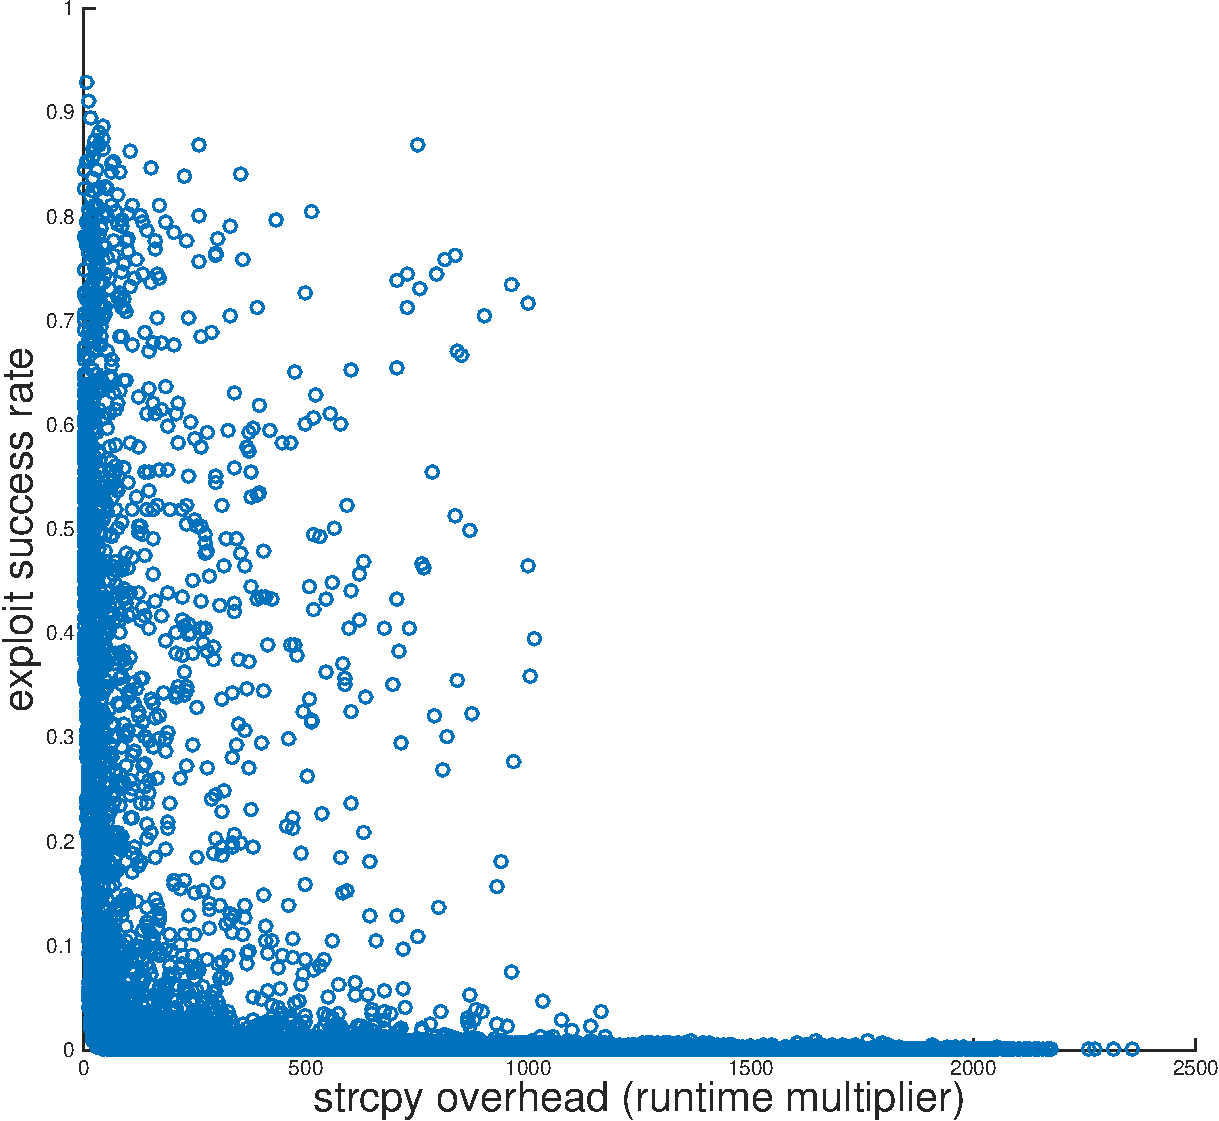
\includegraphics[width=\columnwidth]{successrate.pdf}
%\caption{Graph of exploit success rates with a given strcpy overhead}
%\label{fig_successrate}
%\end{figure}
%
%\begin{figure}
%\centering
%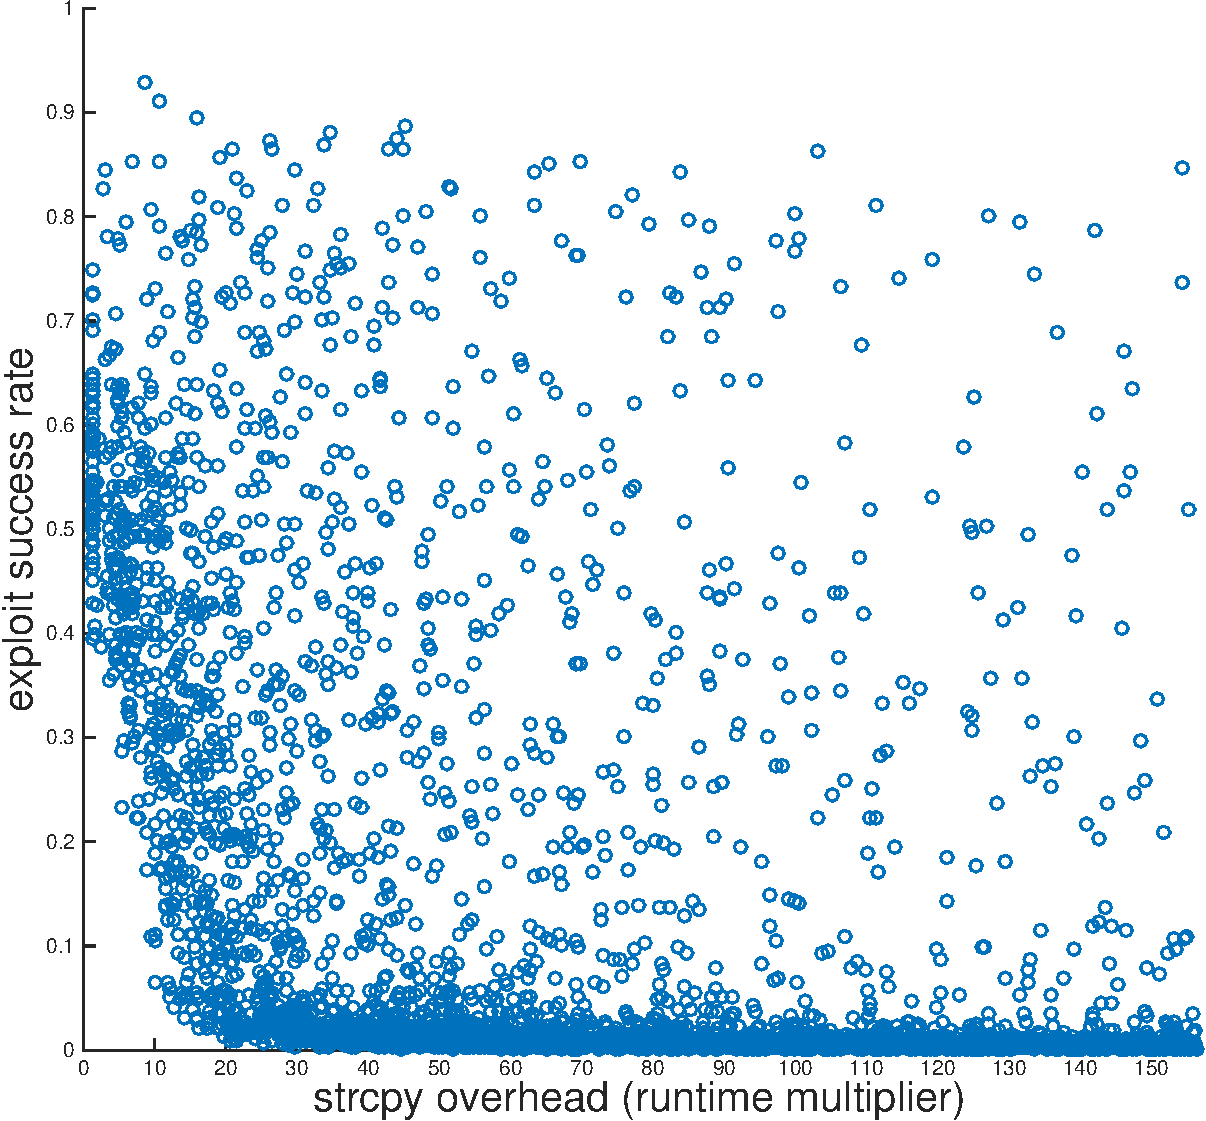
\includegraphics[width=\columnwidth]{successratezoom.pdf}
%\caption{Same graph as Figure \ref{fig_successrate} with strcpy overhead limited to 150\%}
%\label{fig_successratezoom}
%\end{figure}
%
%\begin{figure*}
%\centering
%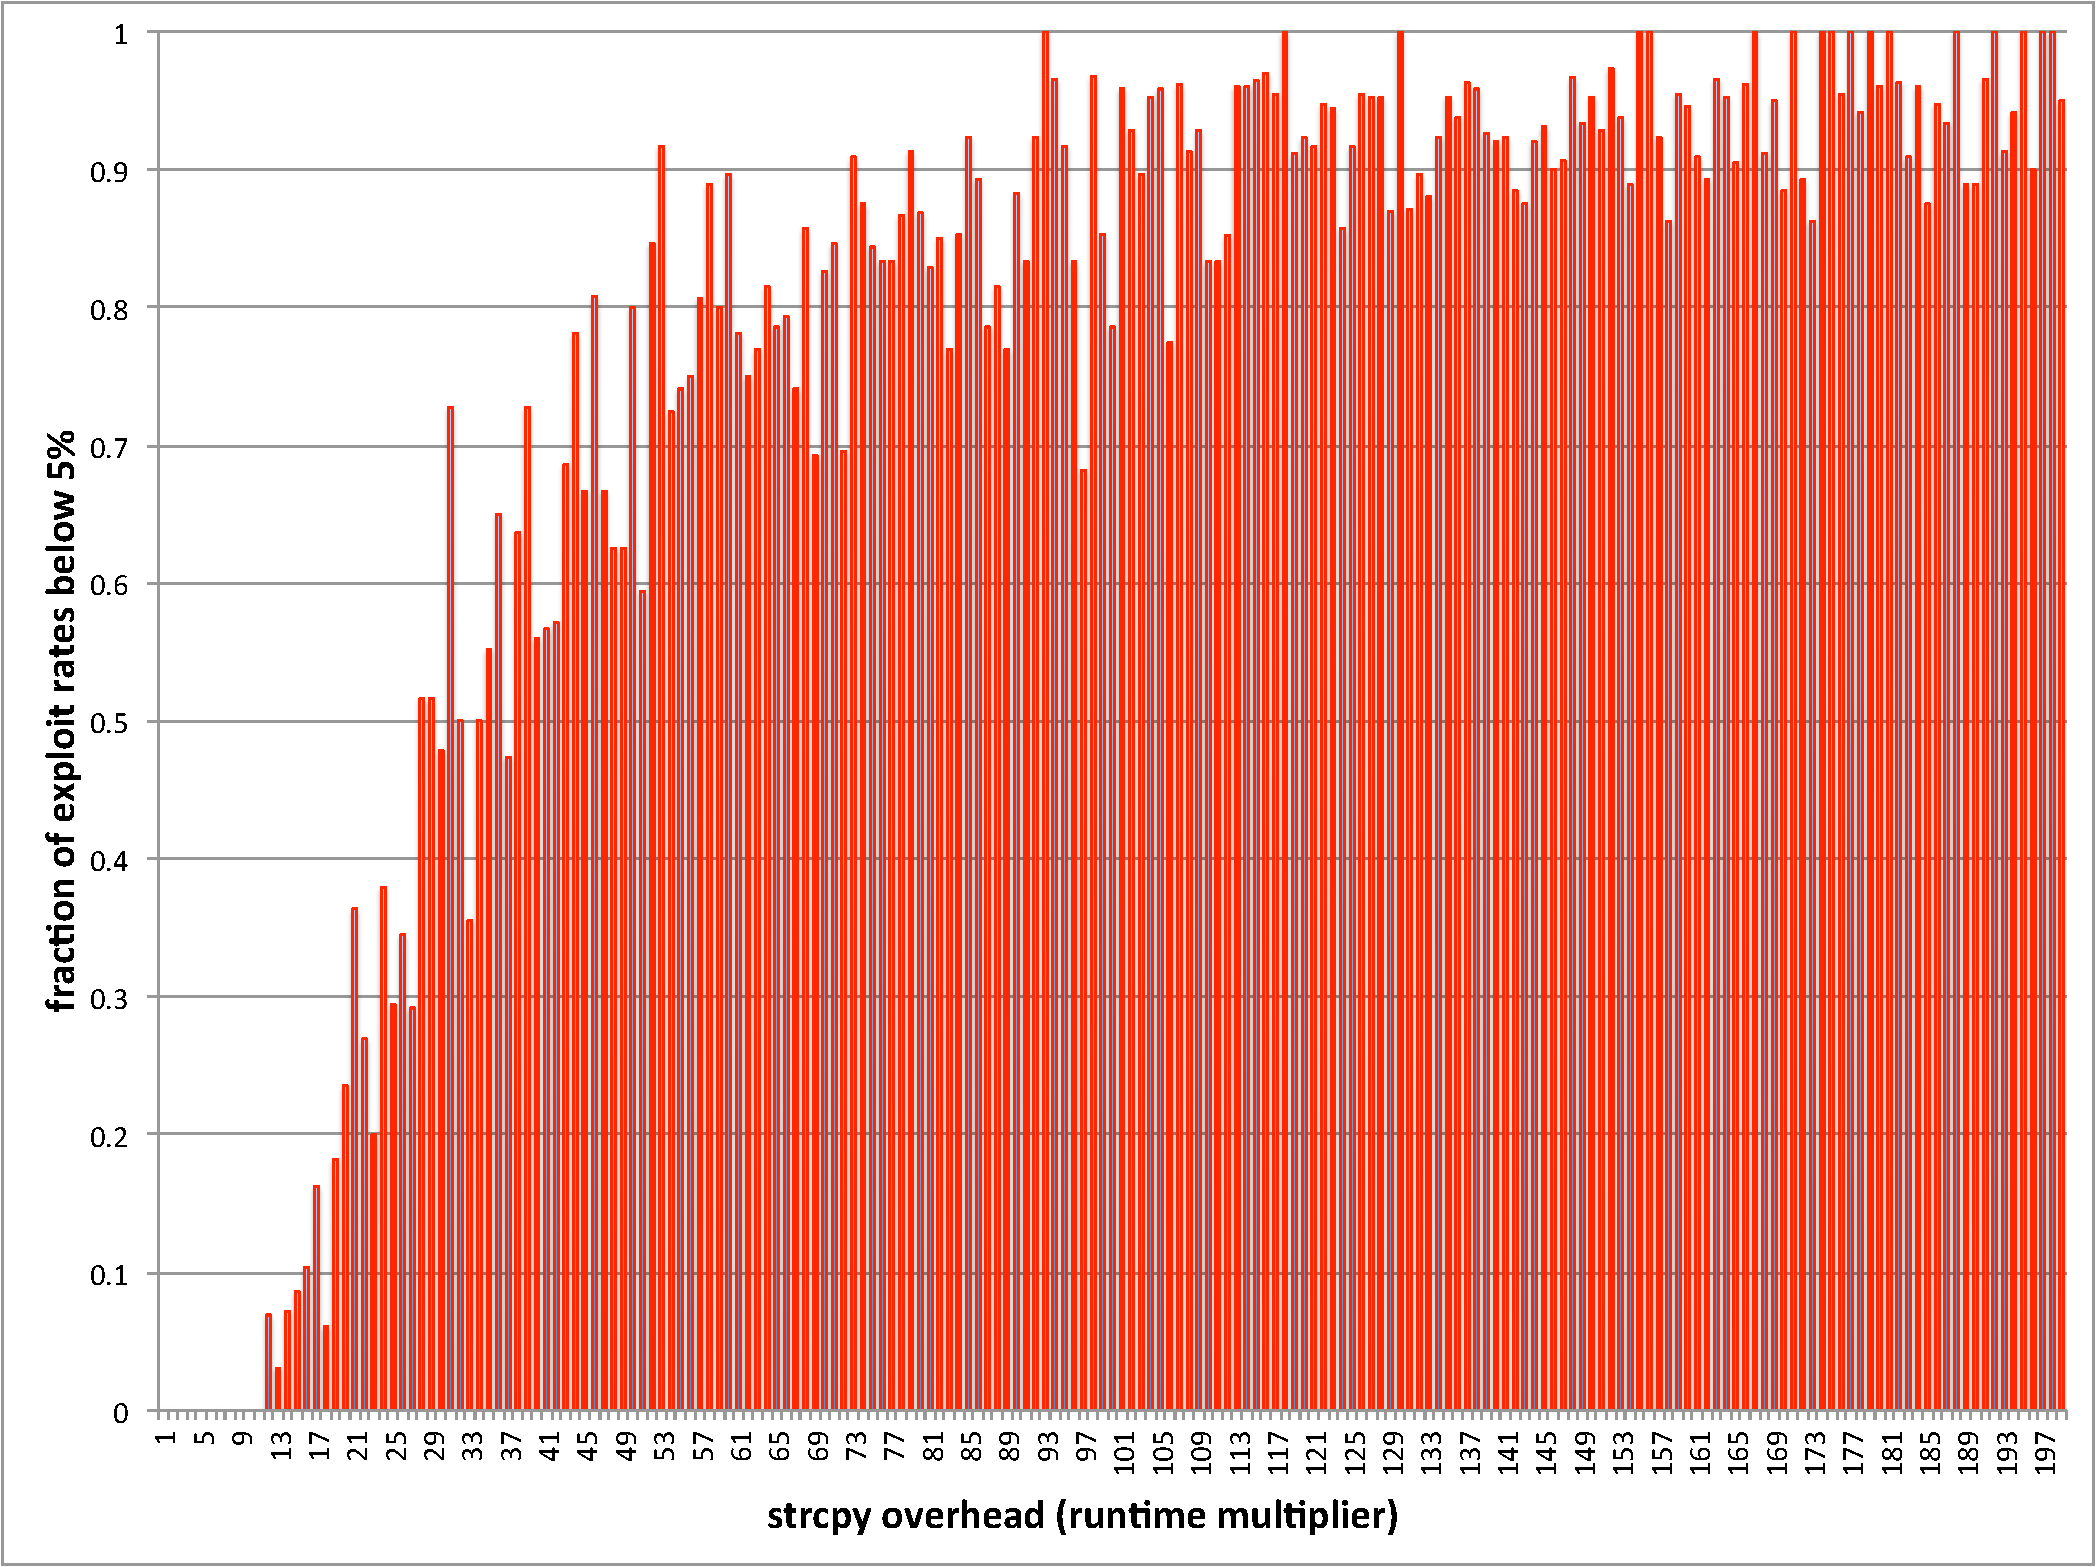
\includegraphics[width=\textwidth]{ratefraction5.pdf}
%\caption{Bar graph of the fraction of exploit success rates under 5\% for a given strcpy overhead}
%\label{fig_ratefraction5}
%\end{figure*}
%The baseline results of the proof-of-concept without library interposition has a runtime of 78 ns and a 99.67\% exploit success rate. Figure \ref{fig_successrate} shows the success rate of exploits with a given \textbf{strcpy} call overhead.  The x-axis shows the overhead of calling \textbf{strcpy} as a runtime multipler.  The y-axis shows the percents of exploits that were successful, or exploits attempts that Libsafe did not caught.  As shown on this graph, as the overhead increases, the exploit success rate decreases.  Eventually as the overhead increases, the success rates plummets down strictly below 10\%.
%
%Figure \ref{fig_successratezoom} shows the same data and has the same x and y axis as Figure \ref{fig_successrate}.  This graph zooms in on the x-axis and limits the runtime mutiplier.  This graph shows that even introducing an runtime mutiplier overhead of 20-30 will decrease the exploit success rate considerably below 10\%.
%
%Figure \ref{fig_ratefraction5} is a bar graph showing the fraction of all exploit success rates that are below 5\% for a given strcpy overhead.  The x-axis is the runtime mutiplier of running \textbf{strcpy} and the y-axis is the fraction of fraction of all exploit success rates that are below 5\%.  A runtime mutltiplier of just 30 is enough to bring the fraction of exploit success rates under 5\% to 0.5.  In other words, half of all exploit success rates are under 5\% when the runtime mutiplier overhead is at 30.  The runtime mutiplier increases with the rate of exploit success rates under 5\%.
%%TODO: Add graphs and mention analysis of graphs
%
%\section{Future Work}
%The next steps are to reduce the overhead associated with time randomization.
%\subsection{Heuristics}
%Introducing heuristics would aid in reducing overhead of function calls.  Identifying certain functions in which time randomization have greater impact, as well as removing time randomization on functions. Instrumenting the next function call after synchronization fuctions, such as pthread library calls, is a possible heuristics.  
%\subsection{Alternative Instrumentation Methods}
%Alternative methods of applying time randomization might aid in reducing function overheads.  Intercepting the function calls made by the binary and introducing delays directly by injecting NOPs will remove the extra steps taken by introducing dynamic library with C code.  Modifying the scheduler is another possible route to add time delays.
%\subsection{Macrobenchmarks}
%This paper analyzes the proof-of-concept exploit as a microbenchmark. However, it is important to determine exploit success rates and overhead introduced to macrobenchmarks as well. Webservers and databases, such as Apache or MySQL, would serve as good macrobenchmarks and indicators of time randomization method on actual systems.
%macrobenchmarks to analyze the effects of time randomization on production or live software.
%
%\section{Conclusion}
%Although we cannot say in the general case that time randomization is an effective method of thwarting concurrency bugs, we have demonstrated that time randomization reduce the effectiveness of the proof-of-concept exploit of CVE-2005-1125.  Further work is required to determine the effectiveness of time randomization on practical or real world systems.
%
%Our current approach using purely random library interposition across all external function calls seems to be too costly in terms of performance.  We will need to improve this performance by implementing heuristics and exploring other methods of adding a time delay.